% ------------------------------------------
%  MASTER THESIS DISSERTATION
% ------------------------------------------
% Author:
%
% Advisors:
%
% ------------------------------------------
\documentclass[10pt,oneside,openright,a4paper]{report}
\usepackage[utf8]{inputenc}

% Set document margins to 1in in all sides
\usepackage[margin=2.5cm]{geometry}
% Line spacing package
\usepackage{graphicx, helvet, hyperref, setspace}
\usepackage[portuguese,english]{babel}
\usepackage[acronym, toc]{glossaries}
% Extra stuff file
% This file is included before begin{document} environment
% Use this to include extra packages and define your own commands
% This way, you can easily grab a most recent version
% of dissertation.tex file from the original repo

\usepackage{float}
\usepackage{xcolor, soul}
\sethlcolor{black}
\newcommand{\Tbullet}[2]{\color{white}\hl{#1} \color{black}\textbf{#2}}

% Built the glossary when the main file is built.
\makeglossaries
% Set main font to Arial
\renewcommand{\familydefault}{\sfdefault}
% Define keywords macro
\providecommand{\keywords}[1]{\textbf{Keywords:} #1}
% Define the NewPage macro
\newcommand*\NewPage{\newpage\null\thispagestyle{empty}\cleardoublepage}
% Abstract-en page numbering
\newcommand {\abstractEnglishPageNumber} {\thispagestyle{plain}\setcounter{page}{\abstractEnglishPage}}
% Abstract-pt page numbering
\newcommand {\abstractPortuguesePageNumber} {\thispagestyle{plain}\setcounter{page}{\abstractPortuguesePage}}
% Section numbering depth
\setcounter{secnumdepth}{2}
% Table of contents depth
\setcounter{tocdepth}{3}
% Set line spacing to 1.5cm
\onehalfspacing
% Page numbering
\pagestyle{plain}

% Glossary-File
% Glossary Definition

\newglossaryentry{MSc}{name={MSc}, description={Masters degree in the area of Science.}}
% Acronym-File
% Acronym Definition
\newacronym{UVE}{UVE}{Unlimited Vector Extension}
\newacronym{SIMD}{SIMD}{Single Instruction Multiple Data}
\newacronym{IST}{IST}{Instituto Superior T\'ecnico}

% ------------------------------------------
% MASTER THESIS DISSERTATION
% ------------------------------------------

\begin{document}
\pagenumbering{gobble}% Remove page numbers (and reset to 1)
\clearpage
\thispagestyle{empty}
%!TEX root = ./dissertation.tex

% Dissertation basic information
\newcommand {\Title} {Novel RISC-V Extension for Data Streaming Complex Patterns}
\newcommand {\Subtitle} {My Subtitle}
\newcommand {\StudentName} {Gonçalo Pinto Midões}
\newcommand {\DegreeName} {Master in Electrical and Computer Engineering}
\newcommand {\Supervisors} {{\large Prof. Pedro Tomás \\\large Prof. Nuno Roma \\\large Prof. Nuno Neves}}

% Include or not include acknowledgments
\def \includeAcknowledgments{1}

% Include or not include glossary
\def \includeGlossary{0}

% Examination Committee
\newcommand {\Chairperson} {{\large Prof./Dr. Lorem Ipsum}}
\newcommand {\Advisor} {{\large Prof./Dr. Lorem Ipsum}}
\newcommand {\CommitteeMembers} {
{\large Prof./Dr. Lorem Ipsum}\\
{\large Prof./Dr. Lorem Ipsum}
}

% Date
\newcommand {\Month} {January}
\newcommand {\Year} {2023}

% Acknowledgments page number
\def \acknowledgmentsPage{1}

% Abstract-en page numbering
\def \abstractEnglishPage{3}

% Abstract-pt page number
\def \abstractPortuguesePage{5}

% You can define your own variables here

%!TEX root = ./dissertation.tex

% ---------------------------------------------------------
%   MASTER THESIS DISSERTATION COVER
% ---------------------------------------------------------
\begin{titlepage}
% ---------------------------------------------------------
%  INSTITUTION LOGO
% ---------------------------------------------------------

\includegraphics[width=5cm]{images/ist_logo}~\\[2.0cm]
\begin{center}
% ---------------------------------------------------------
%  MASTER THESIS DISSERTATION TITLE
% ---------------------------------------------------------
{\LARGE \textbf{\Title}}\\[1.0cm]
% ---------------------------------------------------------
%  MASTER THESIS DISSERTATION SUBTITLE
% ---------------------------------------------------------
%{\Large \Subtitle}\\[1.0cm]
% ---------------------------------------------------------
%  AUTHOR NAME (FULL)
% ---------------------------------------------------------
{\Large \textbf{\StudentName}}\\[1.0cm]
% ---------------------------------------------------------
%  DISSERTATION DEGREE
% -----------------------------------------------------------------
{\large Thesis to obtain the Master of Science Degree in}\\[1.0cm]
% -----------------------------------------------------------------
%  COURSE NAME
% -----------------------------------------------------------------
{\LARGE \textbf{\DegreeName}}\\[1.0cm]

% -----------------------------------------------------------------
%  ADVISORS NAME
% ---------------------------------------------------------
\begin{minipage}[t]{.5\textwidth}
  \begin{flushright}
    {\large Advisor(s)/Supervisor(s):\:}
  \end{flushright}
\end{minipage}%
\begin{minipage}[t]{.5\textwidth}
  \begin{flushleft}
    {\Supervisors}
  \end{flushleft}
\end{minipage}\\[1.0cm]

% ---------------------------------------------------------
%  JURI NAMES:
%  - PRESIDENT
%  - ADVISOR
%  - VOGALS
% ---------------------------------------------------------
{\Large \textbf{Examination Committee}}\\[.25cm]
\begin{minipage}[t]{.5\textwidth}
  \begin{flushright}
    {\large Chairperson:\:}\\
    {\large Advisor:\:}\\
    {\large Members of the Committee:\:}
  \end{flushright}
\end{minipage}%
\begin{minipage}[t]{.5\textwidth}
  \begin{flushleft}
    {\Chairperson}\\
    {\Advisor}\\
    {\CommitteeMembers}
  \end{flushleft}
\end{minipage}\\[1.0cm]

% ---------------------------------------------------------
%  DATE (MONTH AND YEAR)
% ---------------------------------------------------------
{\Large \textbf{\Month\:\Year}}\\
\end{center}
\end{titlepage}
\NewPage

\pagenumbering{roman}

\if\includeAcknowledgments 0
%!TEX root = ../dissertation.tex

% Acknowledgments: This one is optional
\chapter*{Acknowledgments}
% Thanks to everyone and bla bla bla
\NewPage
\fi

%!TEX root = ../dissertation.tex

\begin{otherlanguage}{english}
\begin{abstract}

Your abstract goes here.

% Keywords
\begin{flushleft}

\keywords{my keywords}

\end{flushleft}

\end{abstract}
\end{otherlanguage}
\NewPage

% Table of contents
\tableofcontents
% A new page is necessary only if table of contents has an even number of pages
%\NewPage

% List of tables
%\addcontentsline{toc}{chapter}{\listtablename}
%\listoftables
%\NewPage

% List of figures
%\addcontentsline{toc}{chapter}{\listfigurename}
%\listoffigures
%\NewPage

% List of acronyms
\printglossary[type=\acronymtype]
\NewPage

\pagenumbering{arabic}% Arabic page numbers (and reset to 1)

%!TEX root = ../dissertation.tex

% Entry point for chapters
% In this file you define the order
% in which the chapters are included

% Chapters
%!TEX root = ../dissertation.tex

\chapter{Introduction}
\label{chapter:introduction}

\section{Motivation and Objectives}
\section{Outline of Work}


Your introduction here...\\

A demonstration of how to use acronyms and glossary:

A \gls{MSc} entry.

Second use: \gls{IST}.

Plurals: \glspl{MSc}.

A citation example \cite{nobody}
%!TEX root = ../dissertation.tex

\chapter{State Of The Art}
\label{chapter:state_art}

The growing demand for faster General-Purpose Processors (GPPs)  The improvement of computer speed and capabilities is a very broad area of investigation, with research focused on several areas, from faster computational units, like accelerators, to improvements in data access through pre-fetching, memory caching, and data streaming.



% Data Level paralelism


\section{Unlimited Vector Extention}

Unlimited Vector Extention is a novelty solution that aims to surpass the existing problems of current state-of-the-art solutions of scalable vector extensions, through the use of a data streaming engine, combining streaming and SIMD processing, which allows the exploitation of data parallelism.


The proposed ISA tries to reduce latencies associated with loop control, memory access indexing, and memory access through the use of new instructions that allow a pre-configuration of the stream and the memory access patterns. 
This anticipation of the access control allows for accurate and fast pre-fetching even with multidimensional arrays or indirect memory accesses. 


\subsection{Differentiation}
%The utilization of Single Instruction Multiple Data is not something new, however currently developed approaches focus on operation on fixed-size registers (e.g., Intel MMX, SSE, AVX, etc) this leads to an easier implementation and simplifies hardware requirements. 

%Other solutions have emerged allowing for a more agnostic approach to the physical vector size of registers from the point of view of the programmer. This implementation allows that, only at run time, the compiled software adapts to the given vector size of the system. ARM SVE and RISC-V Vector extension (RVV) are two of these types of implementations.

%The use of any of these solutions incurs the need to modify the active lanes of the vector achieving that through vector control instructions. The addition of these instructions to the iterations leads to an increase in the number of instructions which leads to higher latencies. 

\begin{figure}[H]
    \centering
    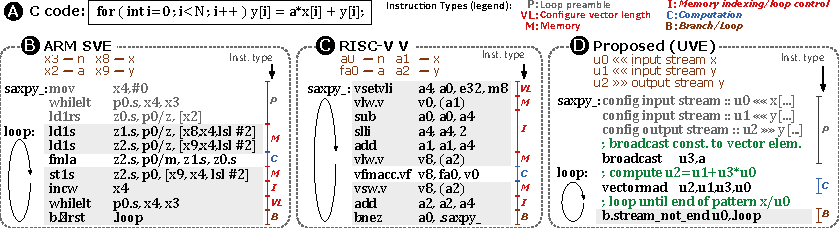
\includegraphics[width=0.77\linewidth]{images/UVE-Comparison.pdf}
    \caption{A boat.}
    \label{fig:uve-comparison}
\end{figure}

The distinguishability of this solution, from  currently developed SIMD solutions (ARM SVE and RISC-V Vector extension (RVV)) comes from features like:
\begin{itemize}
\item[]  \Tbullet{F1}{Decoupled Memory Access} The ability to decouple the memory accesses from the computation part by streaming the data directly to the register allowing the occurrence of loads/stores in parallel with the data manipulation thus reducing the memory access latency.
\item[]  \Tbullet{F2}{Indexing-free Loops} Describing the load/store patterns in advance, minimizing the number of instructions related to memory indexing, reducing the pressure on the processor pipeline (see the UVE Fig.\ref{fig:uve-comparison}.D. It also helps avoid the transfer of miss-predicted data.
\item[]  \Tbullet{F3}{Simpified Vectorization} The description of memory pattern access allows the Streaming Engine to perform all non-coalesced accesses as linear patterns. This leads to a simplified vectorization since memory is always aligned from the execution pipeline point of view - see Fig. \ref{fig:uve-mem-access}. 
\item[]  \Tbullet{F4}{Implicit Load/Store} Due to the description of the streams in the loop preamble, the indexing instructions can be removed meaning that all explicit loads and stores are simply associated with active streams and different vector register.
\end{itemize}

Besides the mentioned features, UVE is also register-size agnostic similar to SVE and RVV, however in UVE there is no need for control instruction since the Streaming Engine automatically disables all vector elements that fall out of bounds, making the loops simpler with a minimal set of control functions.


\begin{figure}[H]
	\begin{center}
 		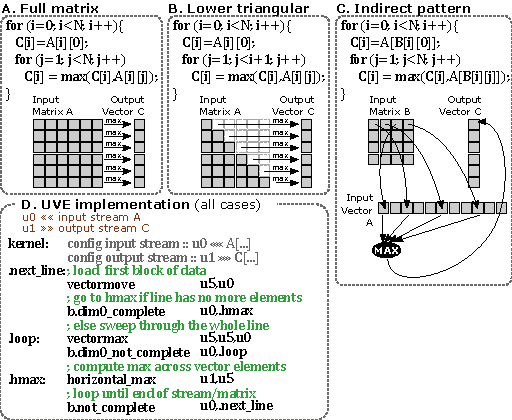
\includegraphics[width=0.37\linewidth]{images/memory-access.pdf}
 		\caption{Execution time for each configuration}
 		\label{fig:uve-mem-access}
	\end{center} 
\end{figure}

\subsection{Data Streaming}

The proposed UVE 



\section{ARM Scalable Vector Extention}
\section{Data-Prefetching}
\section{Stream Specialized Processor}
\section{Stream Semantic Registers}

% Data Streaming
% Memory Vectorization
%!TEX root = ../dissertation.tex

\chapter{Work Plan}
\label{chapter:work_plan}

% Fazer introdução e explicar brevemente o que é o RISC-V, o CVA6

\section{RISC-V UVE Support}
\section{Proposed Architecture}
\section{CVA6 Implementation of Purposed Streaming Engine }
\section{Preliminary Tests on CVA6}
\chapter{Conclusion}
This report highlights the need for further research aiming at the achievement of faster and more capable computer systems. This research can occur in multiple research directions and may involve several improvements in multiple components of the \acrshort{CPU} in order to solve the existing performance bottlenecks.

One of the most relevant problems is related to the manipulation of data utilized by the processor, since it can have a big impact in some modern work fields like Machine Learning, AI, and image and video processing. Leveraging the benefits of advanced memory manipulation strategies like data prefetching, data streaming or vector/SIMD operations is going to be essential to provide \acrfull{GPP} with the improved performance and efficiency that modern workloads and applications require.

The proposed work to be developed during this thesis focuses on implementing and evaluating the performance of the novelty solution of UVE with Data Streaming Support on the CVA6 6-stage CPU. The first step will be to experiment and define the implementation of the proposed streaming engine on the CPU pipeline with the added modifications to all associated functional units and required signals and data structures. After finalizing the hardware description of this modified CPU, a series of tests will be conducted to evaluate several characteristics of the system, like performance, efficiency, and footprint. 

At the end of this thesis, the work developed is expected to provide a new set of tools for further research and improvements on UVE with Data Streaming Support.








\begin{landscape}

\begin{figure}

\section{Gantt Chart}
    
   
\definecolor{groupblue}{RGB}{0, 157, 224}
\definecolor{barblue}{RGB}{173, 216, 230}
\resizebox{1.55\textwidth}{!}{
\begin{ganttchart}[vgrid={draw=none, dotted},%
            %today=15,%
            %today offset=.5,%
            %today label=Heute,%
            %progress=today,%
            y unit title=0.7cm,
            y unit chart=0.6cm,
            bar incomplete/.append style={fill=red},%
            progress label text=  {\quad\pgfmathprintnumber[precision=0,verbatim]{#1}\%}%
            ]{1}{28}
\gantttitle[]{Streaming Complex
Data Patterns on CVA6 Processor}{28}\\
\gantttitle[]{2023}{8}                
    \gantttitle[]{2024}{20}\\
    \gantttitle{Sep}{2}                    
    \gantttitle{Oct}{2}
    \gantttitle{Nov}{2}
    \gantttitle{Dec}{2}
    \gantttitle{Jan}{2}
    \gantttitle{Feb}{2}
    \gantttitle{Mar}{2}
    \gantttitle{Apr}{2}
    \gantttitle{May}{2}
    \gantttitle{Jun}{2}
    \gantttitle{Jul}{2}
    \gantttitle{Aug}{2}
    \gantttitle{Sep}{2}
    \gantttitle{Oct}{2} \\
  \ganttbar[bar/.append style={fill=barblue}]{Work enviroment configuration}{1}{7} \\
  
  \ganttbar[bar/.append style={fill=barblue}]{Writting the report}{6}{9} \\
%%%%%%%%%%%%%%%%%% 2024 %%%%%%%%%%%%%%%%%%%%%%
  
  \ganttbar[bar/.append style={fill=groupblue}] {\textbf{Proposed Architeture Definition and Consolidation}}{11}{13} \\

  \ganttbar[bar/.append style={fill=barblue}] {Analysis of the CVA6 memory interface}{11}{13} \\
  
  
  \ganttbar[bar/.append style={fill=groupblue}]{\textbf{Modification of CVA6 for UVE support with data streaming engine}}{11}{17} \\
  \ganttbar[bar/.append style={fill=barblue}]{Extension of deconding units}{5}{14} \\
  \ganttbar[bar/.append style={fill=barblue}]{Implementation of streaming engine units}{14}{17} \\

  
  \ganttbar[bar/.append style={fill=groupblue}] {\textbf{Design of workload test for the modified CVA6}}{17}{18} \\
  
  \ganttbar[bar/.append style={fill=groupblue}] {\textbf{Execution of tests on developed system}}{18}{22} \\
  
 \ganttbar[bar/.append style={fill=groupblue}] {\textbf{Analysis and Comparison of results}}{20}{23} \\
 
 \ganttbar[bar/.append style={fill=groupblue}] {\textbf{Thesis Writing}}{9}{28} \\
 
 \ganttbar[bar/.append style={fill=barblue}]{Restructure, correction and adaption of work from PIC2 to Master Thesis report}{9}{28} \\
 \ganttbar[bar/.append style={fill=barblue}]{Reporting about the defined ISA Extention and implemented architecture on the CVA6}{17}{28} \\
 \ganttbar[bar/.append style={fill=barblue}]{Writing of comparisons, analysis and conclusions}{23}{28} 
  
\end{ganttchart}
}
 \caption{Gantt chart of the proposed work plan}
\label{fig:ganttchart}
\end{figure}
\end{landscape}


\bibliographystyle{ieeetr}
\addcontentsline{toc}{chapter}{Bibliography}
\bibliography{bibliography/dissertation}


% Glossary and Acronym List
%\if\includeGlossary 1
%\printglossary
%\fi

\end{document}